\section{Simulazioni Monte-Carlo}

L'obiettivo di questa sezione è l'introduzione di tecniche Monte-Carlo che consentano di simulare un modello di Ising con 
numero di costituenti finito. I reticoli considerati sono dotati di condizioni periodiche al contorno, in modo tale che gli spin 
posti agli estremi interagiscano fra loro come primi vicini. Dato che in questo modo tutti gli spin sono equivalenti fra loro ed 
il sistema è invariante per traslazioni, stiamo in pratica simulando un sistema infinito, con un conseguente netto miglioramento 
nella qualità dei risultati. 





\subsection{Generatore di numeri casuali}

Dato che i metodi Monte-Carlo sono una classe di algoritmi numerici che si basano sull'utilizzo di numeri pseudo-casuali, è auspicabile lavorare 
con un generatore dotato di un lungo periodo di generazione. Inoltre il generatore deve essere efficiente, in modo da mantenere contenute le 
tempistiche computazionali. Le simulazioni che hanno portato ai risultati presenti in questa dispensa sono state effettuate con un 
generatore della famiglia PCG \cite{pcg2014}, di cui è riportata l'implementazione. Il linguaggio utilizzato è il Nim, che compila 
direttamente in codice macchina (alte prestazioni), ma presenta una sintassi molto semplice, che ricorda quella del Python.


\begin{minted}[frame=lines, fontsize=\small, bgcolor=blue!10, breaklines = true]{nim}
type 
    PCG* = tuple[state, incr: uint64] ##\
    ## The `PCG` type represents the state of a Permuted Congruential 
    ## Generator (PCG), a family of simple fast space-efficient statistically 
    ## good algorithms for random number generation.

    RandomSetUp* = tuple[inState, inSeq: uint64] ##\
    ## The `RandomSetUp` type is used to initialize a `PCG` generator.


proc random*(gen: var PCG): uint64 =
    ## Get a random uint64 from a `PCG`.

    var 
        oldstate = gen.state
        xorshift = uint32(((oldstate shr 18) xor oldstate) shr 27)
        rot = int32(oldstate shr 59)

    gen.state = oldstate * uint64(6364136223846793005) + gen.incr
    result = ((xorshift shr rot) or (xorshift shl ((-rot) and 31)))


proc newRandomSetUp*(rg: var PCG): RandomSetUp {.inline.} = 
    ## Create a new `RandomSetUp` from a `PCG`.
    (rg.random, rg.random)


proc newPCG*(setUp: RandomSetUp): PCG = 
    ## Create a new `PCG` with the given `RandomSetUp`.

    (result.state, result.incr) = (0.uint64, (setUp.inSeq shl 1) or 1)
    discard result.random
    result.state += setUp.inState
    discard result.random


proc rand*(pcg: var PCG): float32 =
    ## Get a random float32 uniformly distributed over the interval (0, 1)
    pcg.random.float32 / 0xffffffff.float32

proc rand*(pcg: var PCG; a, b: float32): float32 =
    ## Get a random float32 uniformly distributed over the interval (a, b)
    a + pcg.rand * (b - a)
\end{minted}    

I numeri pseudo-casuali vengono generati lavorando con interi senza segno, che consentono di fare operazioni fra bit molto efficienti. 
La corretta implementazione è stata testata imponendo un particolare RandomSetUp e valutando la sequenza generata. 





\subsection{Inizializzazione}

Il primo step della simulazione consiste nel definire una condizione iniziale. Solitamente le scelte più comuni sono la configurazione 
a temperatura nulla (con tutti gli spin allineati) oppure quella a temperatura infinita (con momenti magnetici orientati casualmente). 
Chiaramente tale condizione iniziale non è all'equilibrio per la temperatura alla quale si vuole simulare il sistema. Sarà necessaria 
una fase di termalizzazione in cui il reticolo si rilassa fino a giungere all'equilibrio termodinamico, dopo la quale sarà poi possibile 
iniziare a misurare le osservabili di nostro interesse. Per procedere nello studio del modello è quindi necessario introdurre dei metodi 
che consentano di generare una nuova configurazione e quindi di evolvere il sistema. Le simulazioni riportate in questa dispensa 
hanno fatto uso dell'\textit{algoritmo di Metropolis} e dell'\textit{algoritmo di Wolff}.





\subsection{Algoritmo di Metropolis}

Una mossa dell'algoritmo di Metropolis consiste nel selezionare casualmente uno spin del reticolo con l'obiettivo di generare una 
nuova configurazione invertendolo. La differenza in energia fra lo stato di partenza e quello di arrivo determina 
la probabilità d'accettazione della mossa, dato che per l'\textit{algoritmo di Metropolis} \cite{M(RT)2} si ha che 

\begin{equation}
    A\left(\nu\,|\,\mu\right)\,=\,\text{min}\left[1,\,e^{-\beta\left(E_{\nu}\,-\,E_{\mu}\right)}\right]
    \label{eq: Metropolis_1D}
\end{equation}

Chiaramente se la configurazione $\nu$ ha energia inferiore di quella $\mu$, la mossa viene sempre accettata. In caso contrario, è 
possibile che lo spin non venga invertito e che il nuovo elemento della catena di Markov generata dall'algoritmo di Metropolis sia identico 
a quello precedente. Eseguire $N_{spin}$ volte il ciclo precedente, ossia tentare in media un'inversione per spin, equivale ad aver 
completato uno \textit{sweep} del reticolo. Per le successive fasi conviene studiare le osservabili del sistema in funzione degli sweep e 
non delle singole mosse dell'algoritmo di Metropolis: per questo motivo le implementazioni dell'algoritmo riportato in seguito 
eseguono uno sweep a chiamata, ossia tentano ogni volta $N_{spin}$ inversione. Anche in questo caso il codice riportato è in Nim.



\subsubsection{Metropolis Ising 1D}

\begin{minted}[frame=lines, fontsize=\small, bgcolor=blue!10, breaklines = true]{nim}
    proc metropolisMove*(modIsing: var seq[int], rg: var PCG, temp: float32, acc: float32, hmagn: float32, accettate: var int) = 
    # Algoritmo di Metropolis per evolvere il modello di Ising

    # Indice per selezionare lo spin
    var 
        diffE: float32
        ind, prev, next, appo: int


    for i in 0..<len(modIsing):
        ind = int(rg.rand(float32(0), float32(len(modIsing)))) mod len(modIsing)
        prev = if (ind - 1) mod len(modIsing) == -1: len(modIsing)-1 else: (ind - 1) mod len(modIsing)
        next = (ind + 1) mod len(modIsing)

        appo = modIsing[ind]
        diffE = 2 * acc * float32(appo) * float32(modIsing[prev] + modIsing[next]) + 2 * hmagn * float32(appo)

        if diffE < 0:
            modIsing[ind] = -appo
            accettate += 1

        elif rg.rand() < exp(-diffE/temp):
            modIsing[ind] = -appo
            accettate += 1
\end{minted}    



\subsubsection{Metropolis Ising 2D}

\begin{minted}[frame=lines, fontsize=\small, bgcolor=blue!10, breaklines = true]{nim}
    proc metropolisMove*(modIsing: var seq[seq[int]], rg: var PCG, temp: float32, acc: float32, nspin: int, accettate: var int) = 
    # Algoritmo di Metropolis per evolvere il modello di Ising 2D

    # Indice per selezionare lo spin
    var 
        nmove = int(nspin * nspin)
        diffE: float32
        xcoor, ycoor, appo: int
        up, down, left, right: int


    for i in 0..<nmove:

        # Seleziono casualmente uno spin facente parte del modello
        xcoor = int(floor(rg.rand(float32(0), float32(nspin)))) mod nspin
        ycoor = int(floor(rg.rand(float32(0), float32(nspin)))) mod nspin

        # Determino quali sono i primi vicini in questo caso (facendo attenzione a bc)
        down = (ycoor + 1) mod nspin
        right = (xcoor + 1) mod nspin
        up = (ycoor - 1 + nspin) mod nspin
        left = (xcoor - 1 + nspin) mod nspin

        # Calcolo i contributi energetici
        appo = modIsing[xcoor][ycoor]
        diffE = 2 * acc * float32(appo) * float32((modIsing[right][ycoor] + modIsing[left][ycoor] + modIsing[xcoor][up] + modIsing[xcoor][down]))

        if diffE < 0:
            modIsing[xcoor][ycoor] = -appo
            accettate += 1

        elif rg.rand() < exp(-diffE/temp):
            modIsing[xcoor][ycoor] = -appo
            accettate += 1
\end{minted}    

L'unica differenza fra le due implementazioni riportate in precedenza è la gestione delle condizioni al 
contorno, chiaramente più complessa in due dimensioni dato che il numero di primi vicini duplica, passando 
da due a quattro. La struttura in sè dell'algoritmo rimane la stessa. 





\subsubsection{Metropolis Modello XY}

\begin{minted}[frame=lines, fontsize=\small, bgcolor=blue!10, breaklines = true]{nim}
    # Periodic Boundary Conditions
    proc Pbc(n: int, i: int): int =
        if i >= n: return i - n
        if i < 0: return i + n
        return i
      
    # Energia di interazione con i primi vicini
    proc Boltzmann(spin: float, xcoor: int, ycoor: int): float =
        var ene: float = 0.0
      
        ene = -m_J * cos(m_lattice[xcoor][Pbc(m_nspin, ycoor + 1)] - spin)
        ene -= m_J * cos(m_lattice[xcoor][Pbc(m_nspin, ycoor - 1)] - spin)
        ene -= m_J * cos(m_lattice[Pbc(m_nspin, xcoor + 1)][ycoor] - spin)
        ene -= m_J * cos(m_lattice[Pbc(m_nspin, xcoor - 1)][ycoor] - spin)
      
        return ene
    
    # Singola mossa Metropolis
    proc Move() =
        var xcoor, ycoor: int
      
        xcoor = rand(m_nspin - 1)
        ycoor = rand(m_nspin - 1)
      
        let change = random(-m_delta .. m_delta)
        let appo = m_lattice[xcoor][ycoor] + change
        let enei = Boltzmann(m_lattice[xcoor][ycoor], xcoor, ycoor)
        let enef = Boltzmann(appo, xcoor, ycoor)
      
        if enef - enei < 0 or random(1.0) < exp(-m_beta * (enef - enei)):
          m_lattice[xcoor][ycoor] = appo
          inc accettate
    
    # Sweep del reticolo con Metropolis
    proc Sweep() =
        for i in 0 ..< m_nspin * m_nspin:
            Move()
\end{minted}    

In questo caso la mossa proposta è una rotazione casuale dello spin selezionata nell'intervallo $\left(-\delta,\,\delta\right)$. Tale 
parametro viene fissato in modo tale da avere un acceptance rate pari a circa il 50 \%. 


\subsection{Termalizzazione}

Una simulazione Monte-Carlo è detta all'equilibrio nel momento in cui viene correttamente campionato il peso statistico di Boltzmann 
$p\left(\mu\right)$. Se il sistema viene inizializzato in uno dei due stati presentati in precedenza, ossia quello a temperatura 
nulla (con spin paralleli) oppure a $T$ infinita (con spin orientati casualmente up oppure down) e si vuole performare una simulazione a 
temperatura finita, sarà necessario del tempo computazionale prima che venga raggiunto l'equilibrio, poichè sara necessario accettare 
alcune mosse.

Un modo qualitativo per valutare la durata della termalizzazione consiste nel graficare una quantità d'interesse, 
come può essere la magnetizzazione oppure l'energia interna del sistema. Tali osservabili presenteranno una fase di transitorio 
iniziale in cui il sistema si scorrela dalla condizione iniziale, per poi fluttuare attorno ad un valore pressochè costante. Non è 
sempre garantito che si raggiunga l'equilibrio, in quanto è possibile rimanere bloccati in uno stato metastabile per tempistiche 
computazionali relativamente lunghe. Per evitare di valutare in maniera errata la durata della fase di termalizzazione è consigliabile 
eseguire lo stesso processo per diverse condizioni iniziali e per diversi seed del generatore di numeri casuali, in modo da considerare 
diverse traiettorie nello spazio delle fasi. In Figura \ref{fig: term_Ising1D} è riportato la termalizzazione di un modello di Ising 
1D da 3000 spin a temperatura $T\,=\,0.5$: in questo caso dopo circa 500 sweep della catena viene raggiunto l'equilibrio termodinamico.

\begin{figure}[H]
    \centering
    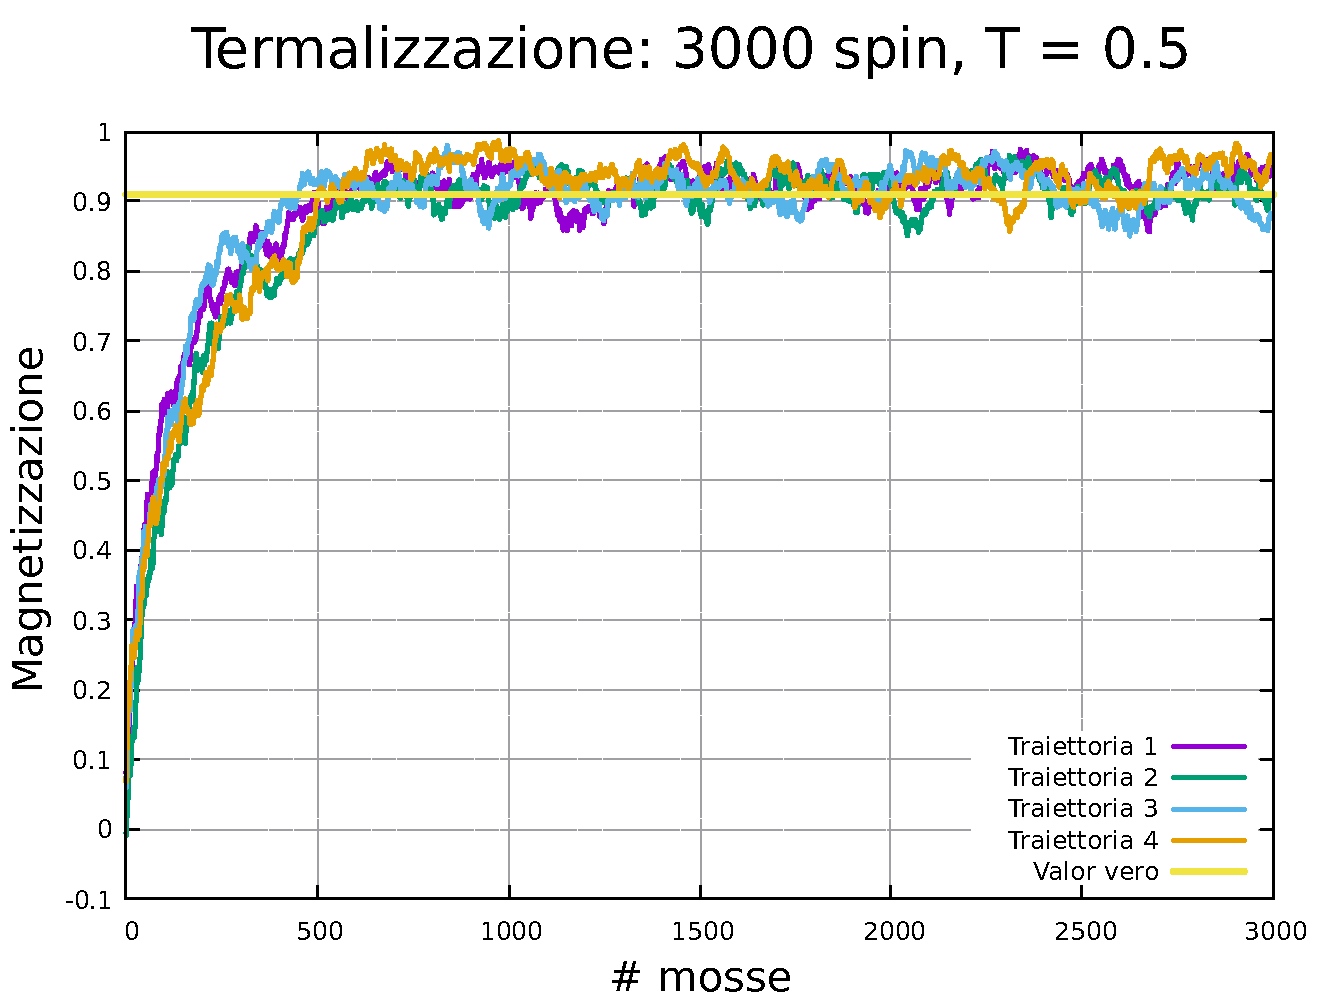
\includegraphics[width=0.6\textwidth]{Immagini/MC_meth/term_3000_0.5.pdf}
    \caption{Termalizzazione per un modello di Ising 1D da 3000 spin a temperatura $T\,=\,0.5$}
    \label{fig: data_block_tech}
\end{figure}



\subsection{Autocorrelazione}

Una volta che il sistema ha raggiunto l'equilibrio, è possibile misurare le osservabili d'interesse senza che i valori d'aspettazione 
siano influenzati dalla fase di transitorio. Per valutare la durata minima della simulazione che consenta di ottenere delle stime 
statisticamente significative è necessaria una misura del tempo di correlazione $t_c$, che esplicita quale sia il numero di sweep 
da effettuare per passare da uno stato ad un altro significativamente differente da quello di partenza. Il modo migliore per 
calcolare $t_c$ consiste nello sfruttare la funzione di autocorrelazione temporale, definita per la magnetizzazione come 

\begin{equation}
    \chi\left(t\right)\,=\,\frac{\left<m\left(t'\right)m\left(t'\,+\,t\right)\right>_{t'}\,-\,\left<m\right>^2}{\sigma^2_m}
    \label{eq: auto_corr_m}
\end{equation}

L'autocorrelazione solitamente presenta una caduta esponenziale con tempo caratteristico pari a quello di correlazione

\begin{equation}
    \chi\left(t\right)\,\sim\,e^{-t/t_c}.
    \label{eq: auto_corr_cad_exp}
\end{equation}

Se si considerano due campioni presi ad un $t_c$ di distanza, la funzione di autocorrelazione assume in presenza di un tale 
intervallo temporale un valore di $1/e$, ancora particolarmente significativo. Se si vuole lavorare con quantità realmente indipendenti 
è necessario campionare a $t\,>\,t_c$; solitamente si impone $t\,=\,2t_c$ in modo che il numero di misure significative in una 
simulazione di durata $t_{max}$ sia pari a 

\begin{equation}
    n\,=\,\frac{t_{max}}{2 t_c}.
    \label{eq: num_ind_samp}
\end{equation}

In Figura \ref{fig: autocorr_Ising_ex} è riportato un esempio di calcolo della funzione di autocorrelazione per un reticolo di spin 
$500 \times 500$ a temperatura pari a due. In questo caso specifico i valori della magnetizzazione sono scorrelati dopo circa 50 sweeps.

\begin{figure}[H]
    \centering
    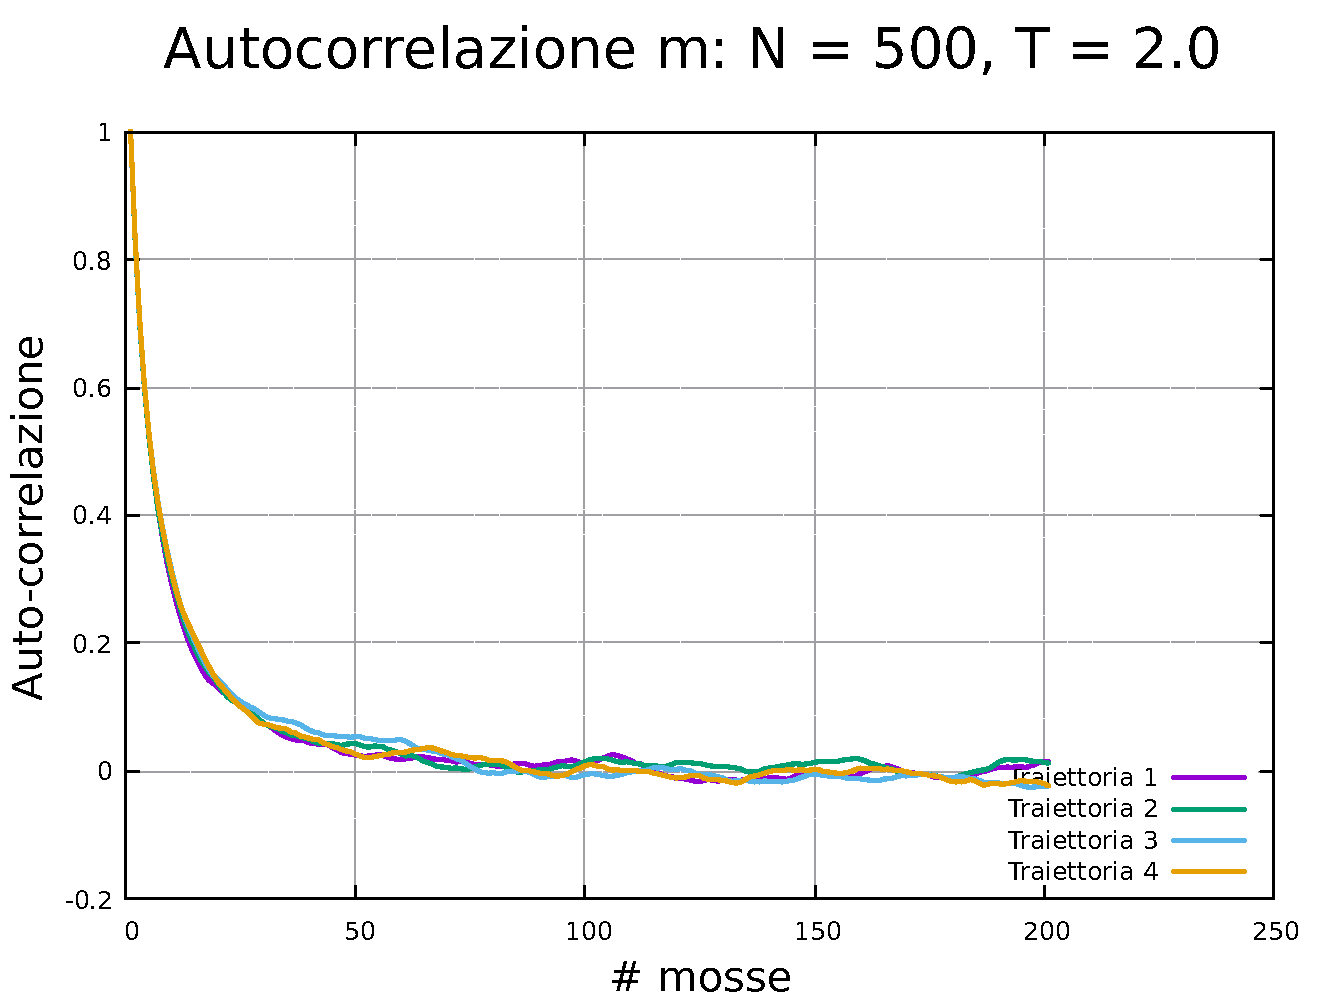
\includegraphics[width=0.6\textwidth]{Immagini/MC_meth/auto_500_2.0.pdf}
    \caption{Autocorrelazione per un modello di Ising 2D di dimensione $500 \times 500$ a temperatura $T\,=\,2.0$}
    \label{fig: autocorr_Ising_ex}
\end{figure}



\subsection{Data-blocking}

Per evitare bias nel campionamento e per ottenere dei valori d'aspettazione adeguati è possibile utilizzare la tecnica del 
data-blocking. Le misure delle osservabili di interesse effettuate durante la simulazione, a distanze temporali inferiori del tempo di correlazione, 
vengono divise in gruppi, per ciascuno dei quali viene calcolato il valor medio. La dispersione di questi valori medi fornisce una 
stima dell'errore associato alla grandezza calcolata. In Figura \ref{fig: data_block_tech} è presentata visivamente la tecnica del 
data-blocking. Le quantità $g_i$ sono le medie di ciascun gruppo.

\begin{figure}[H]
    \centering
    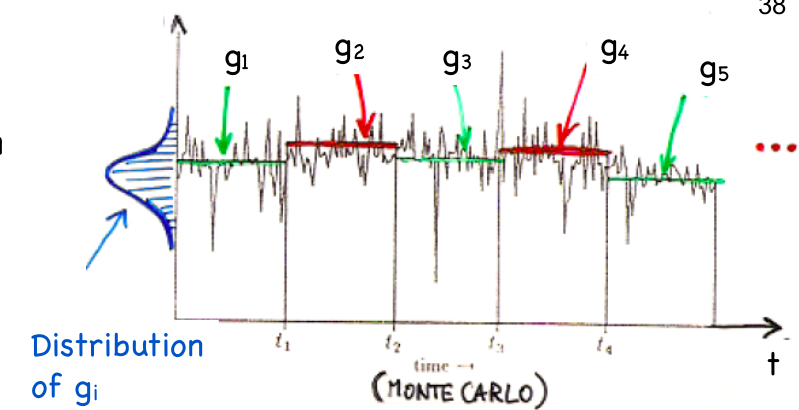
\includegraphics[width=0.6\textwidth]{Immagini/data_blocking.png}
    \caption{Esempio di applicazione della tecnica del data-blocking. Immagine da \cite{galliLSN}.}
    \label{fig: data_block_tech}
\end{figure}

Per determinare quale sia la lunghezza dei blocchi tale da garantire che le medie siano statisticamente indipendenti, si può 
sfruttare il teorema del limite centrale. Nel momento in cui si aumenta la lunghezza dei blocchi, l'errore calcolabile come 

\begin{equation}
    \sigma_{\left<g\right>}\,=\,\sqrt{\frac{1}{N-1}\left(\left<g^2\right>\,-\,\left<g\right>^2\right)}
    \label{eq: error_data_block}
\end{equation}

tende a quello puramente statistico (poichè si va a perdere la correlazione fra le stime) ed oltre una certa lunghezza $L$ dei blocchi 
satura ad un valore costante. La lunghezza di saturazione è la minima accettabile per produrre delle stime adeguate. 
Chiaramente maggiore è il numero di blocchi (della corretta dimensione), migliore sarà la stima finale della osservabile 
d'interesse. In Figura \ref{fig: lblk_exe} è riportato un esempio di stima della dimensione dei blocchi per un reticolo di spin 
$500 \times 500$ a temperatura pari a due. In questo caso specifico possiamo lavorare con blocchi di lunghezza 150 sweeps.

\begin{figure}[H]
    \centering
    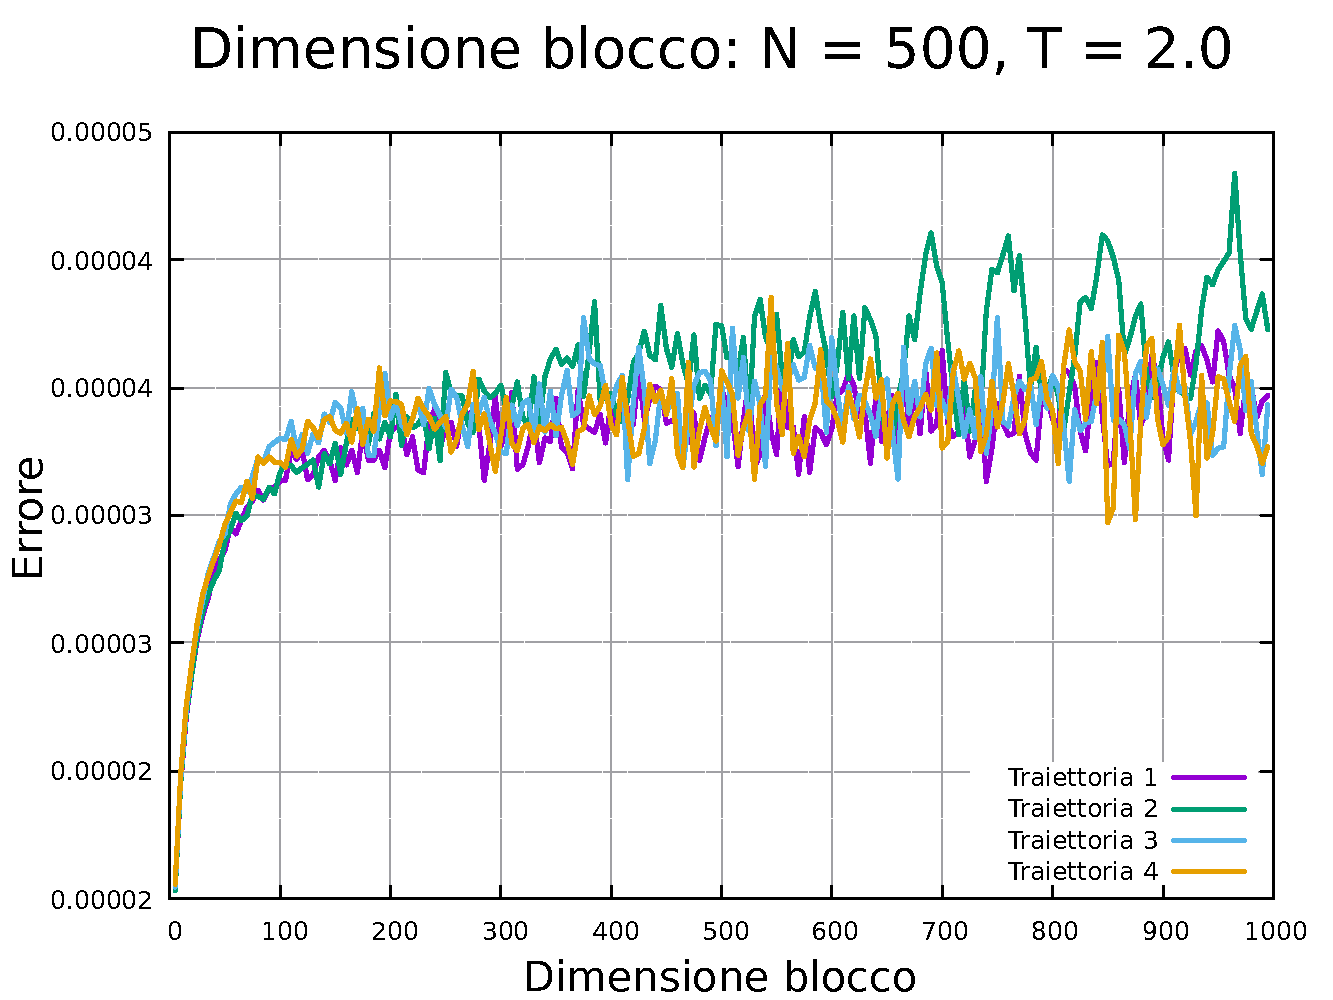
\includegraphics[width=0.6\textwidth]{Immagini/MC_meth/err_500_2.0.pdf}
    \caption{Studio delle dimensioni dei blocchi per un modello di Ising 2D di dimensione $500 \times 500$ a temperatura $T\,=\,2.0$}
    \label{fig: lblk_exe}
\end{figure}





\subsection{Algoritmo di Wolff}

L'algoritmo di Metropolis, anche grazie alla sua semplicità, è il più performante al di fuori della regione 
critica. Tuttavia, quando la temperatura del sistema tende a $T_c$, gli spin tendono a raggrupparsi in 
grandi cluster che contribuiscono significativamente alla magnetizzazione ed all'energia, e nel momento in 
cui cambia l'orientamento degli spin si producono grandi fluttuazioni, note come \textit{fluttuazioni critiche}. 
Questo aspetto, insito nella natura del modello di Ising, comporta un aumento dell'errore statistico 
associato ai valori d'aspettazione degli osservabili, ma è indipendente dall'algoritmo considerato. Un secondo aspetto è legato 
all'aumento della lunghezza di correlazione $\xi$, che nel limite termodinamico diverge alla temperatura critica. Sappiamo che $\xi$ 
è legato al tempo di correlazione dalla relazione 

\begin{equation}
    \tau \propto \xi^z
    \label{eq: tcorr_lcorr}
\end{equation}

Maggiore è $z$, peggio l'algoritmo riesce a generare configurazioni indipendenti fra loro. Per Metropolis, il valore universalmente 
riconosciuto per l'esponente è $z\,=\,2.1665 \pm 0.0012$, che è piuttosto alto \cite{MCM}. Al punto critico, l'algoritmo di Metropolis è vittima 
di \textit{critical slowing down}, dovuto al fatto che è un algoritmo locale (tenta di invertire uno spin alla volta) e quindi non 
riesce a far fronte all'aumento incontrollato della lunghezza di correlazione. Un modo per cercare di ridurre il valore di $z$ è quello 
di lavorare su cluster di spin, in modo tale da invertire contemporaneamente un numero maggiore di spin. L'algoritmo di Wolff, che nelle 
simulazioni qui riportate è stato utilizzato per studiare il punto critico del modello di Ising 2D, sfrutta questa idea e per questo 
motivo fa parte della famiglia degli \textit{algoritmi di clustering}. Uno dei punti cruciali dell'algoritmo consiste nell'identificazione 
del cluster di spin da invertire. La dimensione del blocco dovrebbe dipendere dalla temperatura a cui stiamo simulando il modello, perchè 
per esempio per $T \gg T_c$ gli spin tendono ad essere fra loro scorrelati, evidenziando come dovrebbero essere considerati solo pochi 
momenti magnetici alla volta. L'opposto si può dire del caso a bassa temperatura. Per questo motivo nel momento in cui due spin adiacenti 
hanno lo stesso orientamento non è automatico che essi appartengano allo stesso cluster, ma è presente una certa probabilità di aggiunta 
che aumenta al diminuire della temperatura. Nel caso dell'algoritmo di Wolff, tale probabilità è pari a 

\begin{equation}
    P_{add}\,=\,1\,-\,\exp{\left(-2\beta J\right)}
    \label{eq: padd_cluster}
\end{equation}

In Figura \ref{fig: dim_clW} è riportata la frazione di reticolo ricoperta dal cluster in funzione della temperatura. La probabilità 
introdotta in \eqref{eq: padd_cluster} garantisce la dipendenza corretta al variare della temperatura del modello.

\begin{figure}[H]
    \centering
    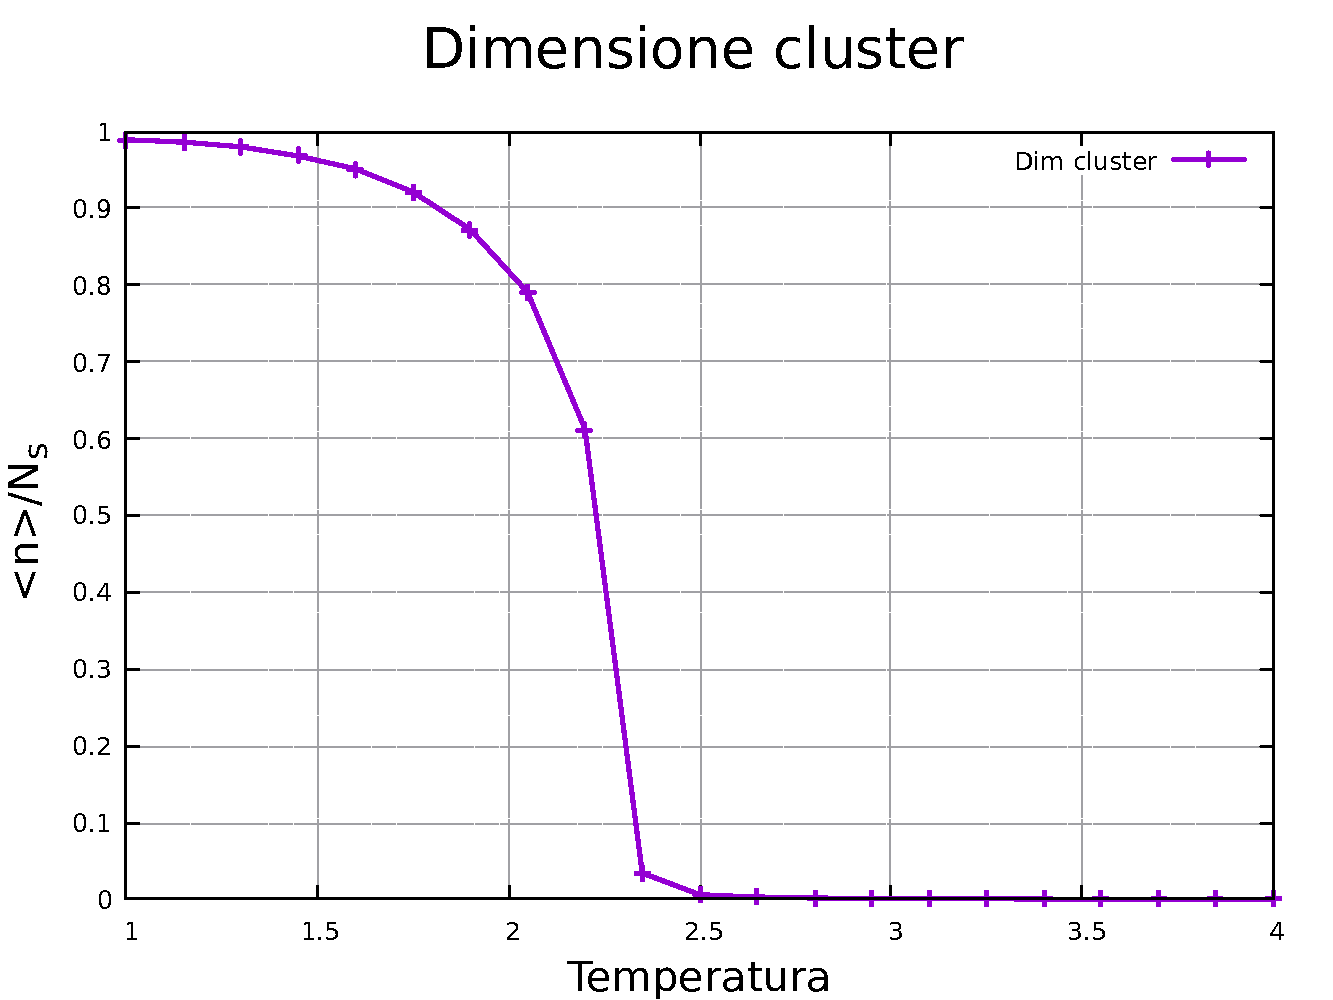
\includegraphics[width=0.75\textwidth]{Immagini/MC_meth/dim_clW.pdf}
    \caption{Frazione di reticolo ricoperta dal cluster in funzione della temperatura.}
    \label{fig: dim_clW}
\end{figure}

L'algoritmo nella sua interezza è costituito dai seguenti passi:

\begin{itemize}[label=$\diamond$] 
    \item si seleziona casualmente uno spin facente parte del reticolo
    \item si prendono in considerazione i primi vicini di quello spin. Se essi sono rivolti nella stessa direzione dello spin 
    selezionato in partenza, aggiungerli al cluster con probabilità data da \eqref{eq: padd_cluster}
    \item per ogni spin che è stato aggiunto allo step precedente, si considerano i primi vicini e si procede con la stessa metodologia. 
    Si continua fino a quando tutti i primi vicini degli spin facenti parte il cluster sono stati presi in considerazione per una possibile 
    inclusione.
    \item si invertono tutti gli spin che costituiscono il cluster. Questo processo avviene con probabilità uno, ossia viene sempre effettuato.
\end{itemize}

Questo algoritmo rispetta sia il bilancio dettagliato che l'ergodicità. La sua particolarità di lavorare su più spin alla volta consente di 
ridurre l'esponente $z$ di un fattore 10, dato che per il modello di Ising 2D è pari a $z\,=\,0.25 \pm 0.01$ \cite{MCM}.


\begin{minted}[frame=lines, fontsize=\small, bgcolor=blue!10, breaklines = true]{nim}
proc wolffMove*(modIsing: var seq[seq[int]], rg: var PCG, temp: float32, acc: float32, nspin: int): int = 
# Algoritmo di Wolff per evolvere il modello di Ising 2D

    var 
        appo: int
        conta: int
        test: IsingCoord
        clusterSize:int = 0
        stack: seq[IsingCoord] = @[]
        padd = 1 - exp(-2*acc/temp)

        # Variabili per coordinate spin
        randSpin, upNeigh, downNeigh, leftNeigh, rightNeigh: IsingCoord

    # Valuto casualmente spin
    randSpin = rg.newRandomCoord(nspin)
    stack.add(randSpin)

    # Salvo valore iniziale spin (per successivi confronti) e poi inverto spin
    appo = modIsing[randSpin.xcoor][randSpin.ycoor]
    modIsing[randSpin.xcoor][randSpin.ycoor] = -appo

    # Continuo fino a quando non ho controllato tutte le possibilità
    while stack.len() > 0:
        test = stack.pop
        clusterSize += 1

        # Valuto quali siano i primi vicini
        upNeigh = newCoord(test.xcoor, (test.ycoor + 1) mod nspin)
        downNeigh = newCoord(test.xcoor, (test.ycoor + nspin - 1) mod nspin)
        leftNeigh = newCoord((test.xcoor + 1) mod nspin, test.ycoor)
        rightNeigh = newCoord((test.xcoor + nspin - 1) mod nspin, test.ycoor)

        # Aggiungo al cluster solo se hanno lo stesso orientamento dello spin di partenza
        if modIsing[upNeigh.xcoor][upNeigh.ycoor] == appo and rg.rand() < padd:
            modIsing[upNeigh.xcoor][upNeigh.ycoor] = -appo
            stack.add(upNeigh)

        if modIsing[downNeigh.xcoor][downNeigh.ycoor] == appo and rg.rand() < padd:
            modIsing[downNeigh.xcoor][downNeigh.ycoor] = -appo
            stack.add(downNeigh)

        if modIsing[rightNeigh.xcoor][rightNeigh.ycoor] == appo and rg.rand() < padd:
            modIsing[rightNeigh.xcoor][rightNeigh.ycoor] = -appo
            stack.add(rightNeigh)

        if modIsing[leftNeigh.xcoor][leftNeigh.ycoor] == appo and rg.rand() < padd:
            modIsing[leftNeigh.xcoor][leftNeigh.ycoor] = -appo
            stack.add(leftNeigh)
    
    return clusterSize
\end{minted}    
    